\documentclass[10pt]{article}
\usepackage{graphicx}
\usepackage[margin=1.5cm]{geometry}
\usepackage{amsmath}
\def\brcurs{{\mbox{$\resizebox{.16in}{.08in}{
\includegraphics{BoldR}}$}}}
\def\rcurs{{\mbox{$\resizebox{.16in}{.08in}{
\includegraphics{ScriptR}}$}}}

\begin{document}
\twocolumn

\title{Thursday Warm-up: Electrostatics}
\author{Prof. Jordan C. Hanson}

\maketitle

\section{Memory Bank}

\begin{itemize}
\item Definition of electric field: $\mathbf{F} = q\mathbf{E}$.
\item Permittivity of free space: $\epsilon_0 = 8.85 \times 10^{-12}$ N$^{-1}$C$^2$m$^{-2}$
\item Let $\rho(\mathbf{r}')$ represent the charge density.
\item Let $Q_{\rm enc} = \int \rho d\tau'$, the total charge within a volume.
\item Coulomb's Law, discrete
\begin{equation}
\mathbf{E}(\mathbf{r}) = \frac{1}{4\pi\epsilon_0}\sum_i \frac{q_i}{\rcurs_i^2}\hat{\brcurs}
\end{equation}
\item Coulomb's Law, continuous
\begin{equation}
\mathbf{E}(\mathbf{r}) = \frac{1}{4\pi\epsilon_0}\int \frac{\rho(\mathbf{r}')}{\rcurs^2}\hat{\brcurs}d\tau'
\end{equation}
\item Gauss' Law, integral form
\begin{equation}
\oint \mathbf{E}) \cdot d\mathbf{a} = \frac{1}{\epsilon_0}Q_{\rm enc}
\end{equation}
\item Gauss' Law, differential form
\begin{equation}
\nabla \cdot \mathbf{E} = \frac{1}{\epsilon_0}\rho
\end{equation}
\end{itemize}

\begin{figure}
\centering
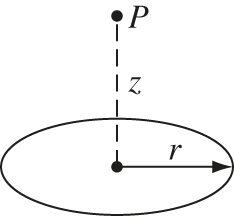
\includegraphics[width=0.15\textwidth]{figures/2_9.jpg} \hspace{0.25cm}
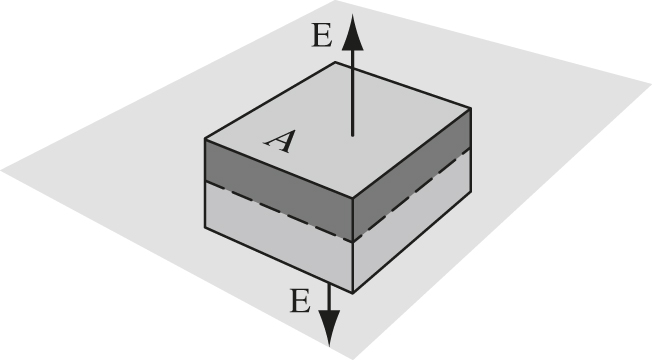
\includegraphics[width=0.25\textwidth]{figures/2_22.jpg}
\caption{\label{fig:1} (Left) A ring of charge, with density $\lambda$.  (Right) An infinite plane of charge, with density $\sigma$.}
\end{figure}

\section{Continuous Charge Distributions}

\begin{enumerate}
\item Consider Fig. \ref{fig:1}, (left).  Find $\mathbf{E}$ at the point $P$, above the ring of charge that lies in the xy-plane, centered at the origin. \\ \vspace{3cm}
\item Consider again Fig. \ref{fig:1}, (left).  Suppose the portion of the ring with $y\geq 0$ was positive, and the portion with $y<0$ was negative.  What is the electric field? \\ \vspace{3cm}
\end{enumerate}

\section{Gauss' Law}

\begin{enumerate}
\item Consider Fig. \ref{fig:1}, (right).  (a) Find $\mathbf{E}$ above the plane of positive charge, with charge density $\sigma$. (b) What is the field below the plane? \\ \vspace{3cm}
\item Imagine a \textit{capacitor}, composed of a two parallel planes of charge, one positive and one negative.  What is the field in the region between them? (b) If the planes are infinitely large, what is the field outside the capacitor? \\ \vspace{3cm}
\end{enumerate}

\section{Review}

\begin{enumerate}
\item If a charge of $q$ and mass $m$ is placed within the capacitor, what is the acceleration of the charge?
\end{enumerate}

\end{document}
